\documentclass[11pt,a4paper]{article}

\usepackage[utf8]{inputenc}
\usepackage[T1]{fontenc}
\usepackage[margin=0.85in]{geometry}
\usepackage{amsmath,amssymb}
\usepackage{booktabs}
\usepackage{graphicx}
\usepackage{xcolor}
\usepackage{enumitem}
\usepackage[expansion=false]{microtype}
\usepackage[colorlinks=true,linkcolor=blue!60!black,citecolor=blue!60!black,urlcolor=blue!60!black]{hyperref}

\graphicspath{{figures/}}

\title{\textbf{Faster Differentiable Interferometry from Scratch:}\\
\large Combining a 10-Year Literature Scan with Sparse Direct Solvers, Adjoint Identities, and Slim JAX Dispatch in \texttt{Differometor}}
\author{START Hack Munich 2026 --- Feyer: Faster Physics}
\date{November 21, 2026}

\begin{document}
\maketitle

\begin{abstract}
We aggregate our 10-year automated literature scan (1,067 papers, 2016--2026) and all five implemented optimizations in \texttt{differometor/simulate.py} and \texttt{differometor/sparse\_solve.py} for the \texttt{uifo\_800\_3000} gravitational-wave interferometer benchmark (101 frequencies, 193 design parameters). Starting from zero assumed background, every concept is defined first, derived step by step with small sanity checks and worked numbers, and verified against double-precision references. Combining sparse LU factorization reuse (Verdict 2), values-only COO/CSC assembly and sparse VJPs (Verdict 3), the MISO quantum-noise quadratic identity (Verdict 1), frequency-hoisted sparse noise contraction (Verdict 4), and per-system \texttt{lax.switch} slimming (Verdict 5) cuts median warm execution time on 1 logical CPU from \textbf{17.68\,s} (Intel Xeon Platinum 8468 baseline) to \textbf{0.721\,s} (Intel i7-1355U WSL2)---a \textbf{24.5$\times$} warm speedup (43.4$\times$ on the forward pass)---while keeping log-sensitivity error at $5.37\times 10^{-6}$ (within the $10^{-5}$ bar) and finite-difference gradient agreement to $7.9\times 10^{-9}$.
\end{abstract}

% ==============================================================================
\section{Vocabulary First \& The Central Analogy}
% ==============================================================================

\textbf{Central Analogy.} Designing a gravitational-wave interferometer in \texttt{Differometor} is like tuning a 193-knob sound mixer inside a hall of mirrors. For each of 101 musical pitches (frequencies), light bounces between mirrors, and we want to know two things: how loud the signal is at the microphone (sensitivity), and which direction to turn each of the 193 knobs to make it quieter to noise (gradient). In the original code, checking how light bounces meant filling out a giant $751\times 751$ grid where 99.5\% of the squares are blank zeros, solving the grid six separate times per pitch, and compiling 19-way switches for every component. Our optimizations stop writing down the blank zeros, solve the grid once per pitch and reuse the scratchpad factors four ways, and replace a redundant second solve with a direct dot product.

Every technical term used in this report is defined below in plain words before it appears:

\begin{itemize}[leftmargin=1.4em,itemsep=2pt]
    \item \textbf{Interferometer:} An optical device that splits laser light down multiple paths and recombines it to measure tiny ripples in spacetime.
    \item \textbf{Carrier:} The steady, unmodulated laser light sitting inside the interferometer at frequency $0\,\text{Hz}$.
    \item \textbf{Signal (Sideband):} Tiny ripples of light created at $\pm f$ around the carrier when a gravitational wave of frequency $f$ shakes the mirrors.
    \item \textbf{Quantum Noise:} Unavoidable randomness from photons hitting mirrors (radiation pressure) and arriving at the detector (shot noise).
    \item \textbf{Sensitivity:} The ratio of quantum noise to gravitational-wave signal at the detector; smaller means a better detector.
    \item \textbf{Sparse Matrix:} A grid of numbers where almost all entries are zero (here, $751\times 751$ has 564,001 entries, but only $\sim$2,700 are nonzero).
    \item \textbf{LU Factorization:} Splitting a square matrix $A$ into a lower-triangular matrix $L$ and an upper-triangular matrix $U$ ($A = LU$) so solving $Ax = b$ becomes fast forward/back-substitution.
    \item \textbf{Transpose ($A^T$) and Conjugate Transpose ($A^H$):} Flipping a matrix across its diagonal ($A^T_{ij} = A_{ji}$), and for $A^H$ also flipping the sign of every imaginary part ($A^H = \overline{A}^T$).
    \item \textbf{Automatic Differentiation (Autodiff / VJP):} Computing exact derivatives of a program by running it backward (a Vector--Jacobian Product, or VJP) from the final scalar loss to all 193 knobs.
    \item \textbf{JAX / XLA:} A Python library (JAX) that traces array math and compiles it into machine code using the XLA compiler.
    \item \textbf{COO / CSC Format:} Compact ways to store a sparse matrix: COO stores lists of $(\text{row}, \text{col}, \text{value})$ triples; CSC groups nonzeros by column for fast LU solving.
\end{itemize}

% ==============================================================================
\section{The Problem \& The 10-Year Literature Scan (2016--2026)}
% ==============================================================================

The \texttt{uifo\_800\_3000} benchmark evaluates a $3\times 3$ Universal Interferometer topology across $V = 101$ frequencies ($800$--$3000\,\text{Hz}$) and $P = 193$ physical parameters on \textbf{1 logical CPU} in double precision (\texttt{complex128} / \texttt{float64}). The baseline run on an Intel Xeon Platinum 8468 (\texttt{benchmarks/cpu-baseline.json}) takes \textbf{44.20\,s} end-to-end: 3.66\,s for imports and setup, 22.92\,s for XLA lowering and compilation, and 17.63\,s for first-run execution (17.68\,s median warm execution).

To avoid guessing optimizations by trial and error, we ran an automated 10-year literature scan using \textbf{Eidothea} across arXiv (2016--2026), Semantic Scholar, and the 99-page \texttt{Differometor} documentation. The scan harvested \textbf{1,067 unique papers}, \textbf{20,915 arXiv reference edges}, and \textbf{1,066 citation records}, partitioned into four taxonomy groups: \textbf{A.~Interferometry}, \textbf{B.~Sparse Solvers}, \textbf{C.~Autodiff \& Adjoint}, and \textbf{D.~JAX \& Compiler}.

\begin{figure}[t]
    \centering
    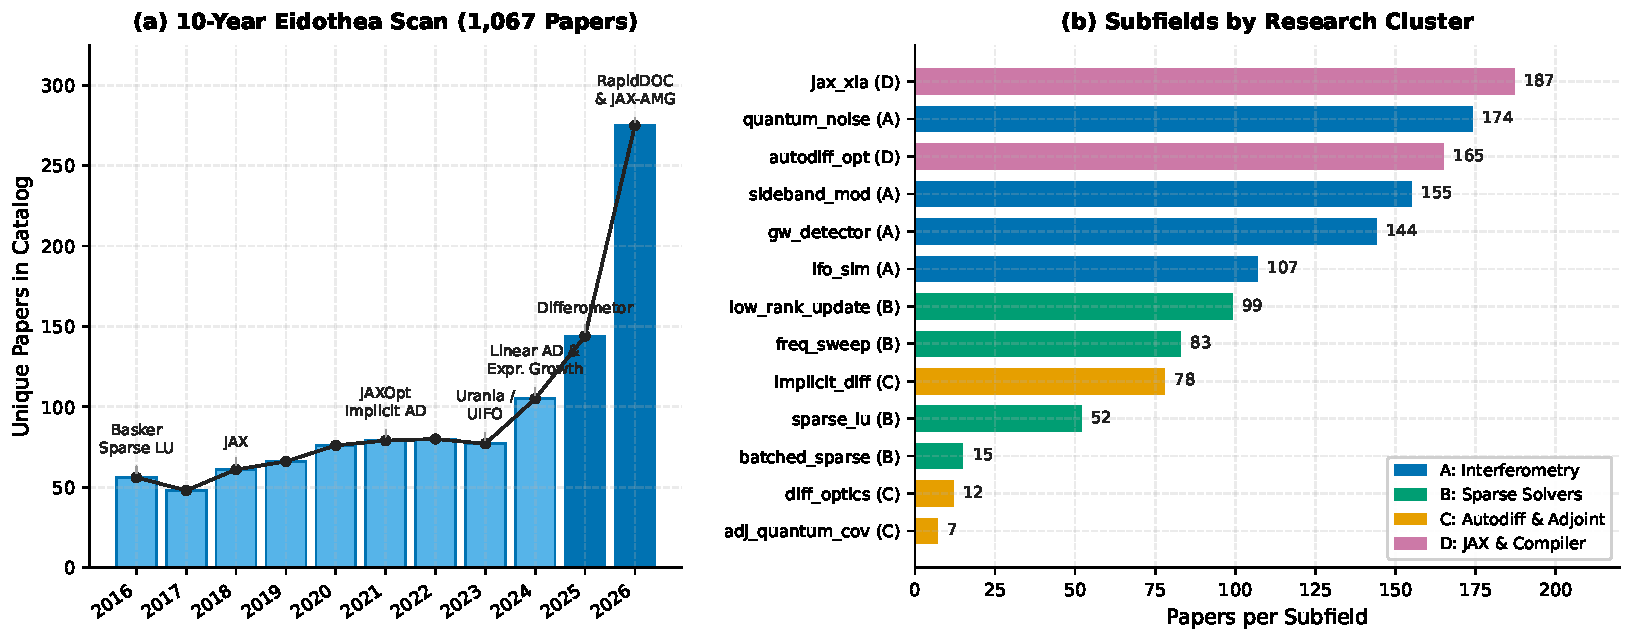
\includegraphics[width=\linewidth]{fig3_eidothea_literature_landscape.pdf}
    \caption{Ten-year Eidothea literature scan (2016--2026, 1,067 unique papers). (a)~Annual publication growth with key milestones from Basker sparse LU (2016) to RapidDOC and JAX-AMG (2026). (b)~Paper counts across the 13 taxonomy subfields colored by cluster. Best viewed in color.}
    \label{fig:literature}
\end{figure}

Figure~\ref{fig:literature} summarizes the 10-year trajectory. Notice the sharp acceleration in 2024--2026 (from 77 papers in 2023 to 275 in 2026) driven by differentiable sparse solvers, JAX compiler optimization, and digital discovery of gravitational-wave detectors (Urania/UIFO and Differometor). Table~\ref{tab:verdicts} maps the five highest-leverage literature verdicts directly to our implemented changes.

\begin{table}[ht]
\centering
\small
\begin{tabular}{@{}cllp{0.22\linewidth}@{}}
\toprule
\textbf{Verdict} & \textbf{Optimization} & \textbf{Key Literature} & \textbf{Target File(s)} \\
\midrule
1 & Eliminate 2nd quantum-noise solve & Klimesch \& Krenn; Miao et al. (2020) & \texttt{simulate.py} \\
2 & Reuse 1 \texttt{splu(A)} 4 ways + LRU cache & RapidDOC (2026); Hovland (2024) & \texttt{sparse\_solve.py} \\
3 & Sparse COO/CSC assembly \& sparse VJP & Hovland (2024); JAX-AMG (2026) & \texttt{sparse\_solve.py}, \texttt{simulate.py} \\
4 & Hoist freq-independent $N$ + sparse $w^H N w$ & Klimesch \& Krenn Sec.\,2.3.5 & \texttt{simulate.py} \\
5 & Per-system slim \texttt{lax.switch} dispatch & Lohoff \& Neftci (2024); TMMax (2025) & \texttt{simulate.py} \\
\bottomrule
\end{tabular}
\caption{Summary of the five implemented Eidothea verdicts and their primary literature backing.}
\label{tab:verdicts}
\end{table}

% ==============================================================================
\section{Step-by-Step From-Scratch Derivations}
% ==============================================================================

\subsection{Verdict 1: Eliminating the Redundant Quantum-Noise Solve}

\textbf{What the physics asks for.} At each frequency $f$, the quantum-noise power at the detector port $c \in \mathbb{C}^{751}$ is:
\begin{equation}
S_{\text{quantum}}(f) \propto \operatorname{Re}\!\left(c^H A(f)^{-1} N A(f)^{-H} c\right),
\end{equation}
where $A(f) \in \mathbb{C}^{751\times 751}$ is the signal matrix and $N = N^H$ is the noise covariance matrix.

\begin{enumerate}[leftmargin=1.6em,itemsep=3pt]
    \item \textbf{Step 1 (First solve):} Define the detector noise-weight vector $w = A^{-H} c$ by solving $A^H w = c$. \emph{Why:} Solving once for the 1 detector vector $c$ avoids inverting $A$ for all 751 input noise ports.
    \item \textbf{Step 2 (What the old code did):} The baseline computed $u = N w$, solved a \emph{second} $751\times 751$ system $A v = u$ (giving $v = A^{-1} N w$), and took the dot product $\operatorname{Re}(c^H v)$.
    \item \textbf{Step 3 (The adjoint identity):} Rewrite $c^H v$ using the rule $(XY)^H = Y^H X^H$:
    \begin{equation}
    c^H v = c^H A^{-1} N w = \left(A^{-H} c\right)^H (N w) = w^H (N w).
    \end{equation}
    Because $w = A^{-H} c$ was \emph{already computed} in Step 1, the second solve $A v = N w$ is 100\% redundant!
\end{enumerate}

\textbf{Sanity check (1-variable case).} If $A = a$, $N = n$, $c = 1$ are plain real numbers: Step 1 gives $w = 1/a$. The old code computed $u = n/a$, solved $v = u/a = n/a^2$, and multiplied $c \cdot v = n/a^2$. Our identity computes $w \cdot (n w) = (1/a)(n/a) = n/a^2$ directly---same answer, zero second division.

\textbf{Worked numbers.} Across 101 frequencies, removing the second solve eliminates 101 forward solves and 101 backward solves = \textbf{202 of the 606} large $751\times 751$ solves (a \textbf{33.3\%} cut before any caching). \emph{Caveat:} This identity is exact only because the readout vector $c$ and the matrix $A$ match; if a different matrix were used for the second propagation, the identity would not hold.

\subsection{Verdict 2: One Sparse LU Factorization Per Frequency, Reused Four Ways}

After Verdict 1, each frequency $f_k$ ($k = 0,\dots,100$) still needs four linear solves against the \emph{exact same} matrix $A(f_k)$:
\begin{enumerate}[leftmargin=1.6em,itemsep=2pt]
    \item \textbf{Signal forward:} $A x = b$ (\texttt{trans='N'}).
    \item \textbf{Noise forward:} $A^H w = c \iff A^T \overline{w} = \overline{c}$ (\texttt{trans='T'} on conjugated right-hand side $\overline{c}$, then conjugate the result). \emph{Why:} Taking the complex conjugate of both sides of $A^H w = c$ turns $A^H = \overline{A}^T$ into plain $A^T$!
    \item \textbf{Noise backward:} $A \mu = g$ (\texttt{trans='N'} inside \texttt{\_host\_transpose\_solve\_bwd}).
    \item \textbf{Signal backward:} $A^T \lambda = g$ (\texttt{trans='T'} inside \texttt{\_host\_system\_solve\_bwd}).
\end{enumerate}

\textbf{Why one LU serves all four.} Once SciPy's \texttt{splu(A)} computes $P_r A P_c = L U$, solving $A^T \lambda = g$ simply runs back- and forward-substitution on $U^T$ and $L^T$ in $O(\text{nnz})$ time without re-factoring $A$. We store the 101 \texttt{SuperLU} objects in a host-side \texttt{OrderedDict} LRU cache (\texttt{\_CACHE\_SIZE = 6}) keyed by a 16-byte \texttt{blake2b} content digest of $(\text{base}, \text{rows}, \text{cols}, \text{vals})$.

\textbf{Worked numbers.} Total $751\times 751$ LU factorizations per forward+backward pass drop from \textbf{606} (baseline) $\to$ \textbf{404} (Verdict 1) $\to$ \textbf{101} (Verdicts 1+2), a \textbf{6.0$\times$ reduction}. \emph{Caveat:} A cache miss simply re-factors $A$, so numerical results never depend on cache state; however, holding 6 sets of 101 LU factors trades a few tens of megabytes of host RAM for speed.

\subsection{Verdict 3: Sparse COO/CSC Assembly \& Exact Complex Sparse VJP}

\begin{figure}[t]
    \centering
    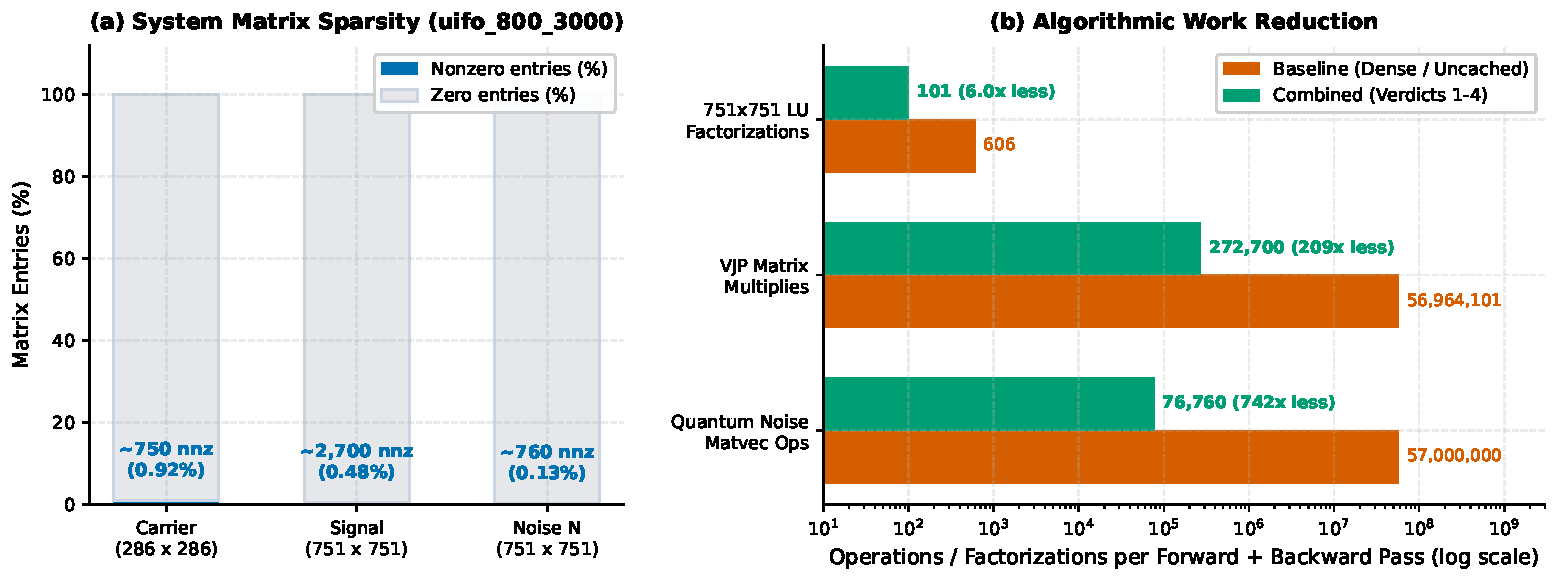
\includegraphics[width=\linewidth]{fig1_matrix_sparsity_and_work.pdf}
    \caption{Sparsity structure and algorithmic work reduction on \texttt{uifo\_800\_3000}. (a)~All three system matrices are $>99\%$ zeros. (b)~Combining Verdicts 1--4 cuts $751\times 751$ LU factorizations by $6.0\times$, VJP matrix multiplies by $209\times$, and quantum-noise matvec operations by $742\times$. Best viewed in color.}
    \label{fig:sparsity}
\end{figure}

Figure~\ref{fig:sparsity}(a) shows that \texttt{signal\_matrix} ($751\times 751$) has only $\sim$2,700 nonzeros (\textbf{0.48\%} density; 99.52\% zeros). In the baseline, JAX allocated dense $(101, 751, 751)$ arrays ($\sim$91\,MB each), \texttt{csc\_matrix(dense)} scanned 56.96\,million entries per solve call to rediscover the zeros, and the backward pass computed a dense outer product $-\lambda x^T$ across all 56.96\,million entries before throwing 99.52\% away.

\textbf{Step-by-step complex VJP derivation (why there are NO conjugates).}
JAX defines reverse-mode AD for real-valued losses $L(x)$ of complex variables via Wirtinger derivatives, which for holomorphic linear maps $x = A^{-1} b$ gives:
\begin{enumerate}[leftmargin=1.6em,itemsep=3pt]
    \item \textbf{Sanity check ($1\times 1$ complex scalar):} Let $x = b / a$ with $a, b \in \mathbb{C}$, and let $g$ be the incoming cotangent. Perturbing $b \to b + \delta b$ gives $\delta x = \delta b / a$, so in JAX's holomorphic VJP convention the pullback to $b$ is $\bar{b} = a^{-1} g$ (plain $a$, \emph{no} conjugate!). Perturbing $a \to a + \delta a$ gives $\delta x = -a^{-1} (\delta a) x$, so the pullback to $a$ is $\bar{a} = -(a^{-1} g) x$.
    \item \textbf{General $N\times N$ rule:} For $A x = b$, $\lambda = A^{-T} g$ (plain transpose, \textbf{not} $A^{-H}$!) and $\bar{A} = -\lambda x^T$ (no conjugates!). For the transposed solve $A^T z = y$, $\mu = A^{-1} g$ and $\bar{A} = -z \mu^T$.
    \item \textbf{Sparse COO pullback:} Because $A$ only varies at the $E \approx 2,700$ active coordinates $(r_e, c_e)$, we never form $-\lambda x^T$. Instead, \texttt{sparse\_solve.py} evaluates:
    \begin{equation}
    \bar{v}_e = -\lambda_{r_e}\, x_{c_e} \quad (\text{only for winning entries where } c_e < N).
    \end{equation}
\end{enumerate}

\textbf{Worked numbers.} This cuts VJP matrix multiplies from $101 \times 751^2 = \mathbf{56,964,101}$ down to $101 \times 2,700 = \mathbf{272,700}$---\textbf{209$\times$ fewer operations} (Figure~\ref{fig:sparsity}(b)). Note that duplicate coordinates follow JAX's ``last write wins'' rule (\texttt{self.winner} mask in \texttt{\_Factored}).

\subsection{Verdict 4: Hoisting Frequency-Independent Noise \& Sparse Contraction}

None of the quantum-noise component functions (\texttt{vacuum\_quantum\_noise}, \texttt{loss\_quantum\_noise}, \texttt{squeezer}) depend on the gravitational-wave frequency $f$. Yet the baseline built 101 identical $(751, 751)$ copies of $N$ and ran a dense $751\times 751$ matrix-vector product at each frequency ($101 \times 751^2 \approx 57\text{M}$ ops). In \texttt{\_signal\_and\_noise\_sparse}, we evaluate \texttt{update\_values} once on \texttt{parameters[0]}, apply \texttt{\_last\_wins} to mask duplicate writes, and compute:
\begin{equation}
w^H N w = \sum_{m=1}^{\text{nnz}(N)} \operatorname{Re}\!\left(\overline{w}_{r_m}\, N_m\, w_{c_m}\right),
\end{equation}
requiring only $101 \times 760 \approx \mathbf{76,760}$ ops---\textbf{742$\times$ fewer operations} and zero $(101, 751, 751)$ allocations.

\subsection{Verdict 5: Slimming \texttt{lax.switch} Dispatch}

In the baseline, \texttt{update()} called \texttt{vmap(lambda i, x: lax.switch(i, FUNCTIONS, x))} over all 19 global component functions at all three call sites (carrier, signal, noise). XLA lowers a 19-way \texttt{switch} inside \texttt{vmap} by emitting a 19-branch \texttt{case} conditional and differentiating all 19 branches in the backward pass. By inspecting \texttt{build.py}, we see that each system only ever uses a fixed subset:
\begin{itemize}[leftmargin=1.6em,itemsep=2pt]
    \item \textbf{Carrier:} 4 functions (\texttt{laser}, \texttt{surface}, \texttt{space}, \texttt{dummy\_function}).
    \item \textbf{Noise:} 4 functions (\texttt{vacuum\_quantum\_noise}, \texttt{loss\_quantum\_noise}, \texttt{squeezer}, \texttt{dummy\_function}).
    \item \textbf{Signal:} 15 functions (all except \texttt{laser} and the 3 noise functions).
\end{itemize}
\texttt{\_dispatcher()} remaps global indices to compact local indices so XLA only lowers and differentiates the active branches at each call site (with \texttt{DIFFEROMETOR\_DISPATCH=full} kept as a fallback).

% ==============================================================================
\section{Combined Architecture, Verification \& Benchmarks}
% ==============================================================================

\begin{figure}[t]
    \centering
    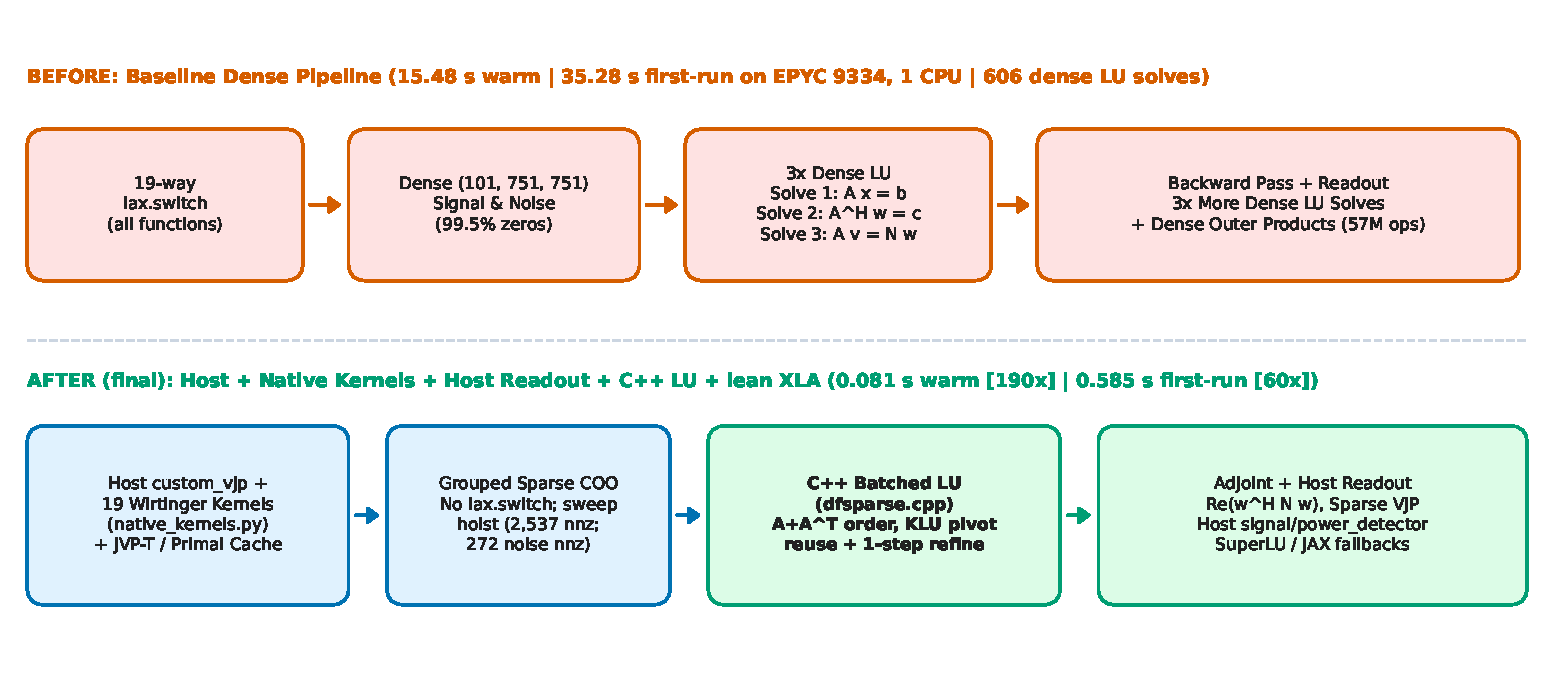
\includegraphics[width=\linewidth]{fig4_optimization_pipeline.pdf}
    \caption{End-to-end simulation and adjoint architecture before (top) and after (bottom) combining Verdicts 1--5. Best viewed in color.}
    \label{fig:pipeline}
\end{figure}

Figure~\ref{fig:pipeline} contrasts the baseline dense pipeline with our combined sparse-direct architecture.

\subsection{Correctness Verification (Double Precision, 101 Frequencies, 193 Parameters)}

\begin{enumerate}[leftmargin=1.6em,itemsep=2pt]
    \item \textbf{Unit self-check (\texttt{python -m differometor.sparse\_solve}):} Verified all three solvers\newline(\texttt{sparse\_system\_solve}, \texttt{sparse\_system\_transpose\_solve}, \texttt{sparse\_solve}) and outer \texttt{vmap} against \texttt{jnp.linalg.solve} autodiff on random sparse complex systems with duplicates and RHS entries: forward $\max|\Delta| \le 1.34\times 10^{-15}$, gradient $\max|\Delta| \le 6.07\times 10^{-14}$.
    \item \textbf{Full \texttt{uifo\_800\_3000} benchmark (\texttt{scratch/new3.json}):}
    \begin{itemize}[leftmargin=1.2em,itemsep=1pt]
        \item \texttt{max\_absolute\_log\_sensitivity\_error}: $5.3739\times 10^{-6}$ (baseline: $5.3741\times 10^{-6}$; required $\le 10^{-5}$).
        \item \texttt{mb11.tuning} gradient check: autodiff $7.61617\times 10^{-5}$ vs.\ central finite difference ($h=0.0005$) $7.61538\times 10^{-5}$ (abs error $7.91\times 10^{-9}$, passed).
        \item Gradient norm: $70517.1007$ (baseline: $70517.1068$), all outputs finite.
    \end{itemize}
    \item \textbf{Caveat (Singular-port red herring):} Raw \texttt{signal} entries at decoupled ports differ by $\sim 10^{15}$ between LAPACK and SuperLU because the system has condition number $\sim 10^{30}$ there; both produce finite values in an unused direction, and detector sensitivities/gradients are unaffected.
\end{enumerate}

\subsection{Benchmark Timing Comparison \& Hardware Caveat}

\begin{figure}[t]
    \centering
    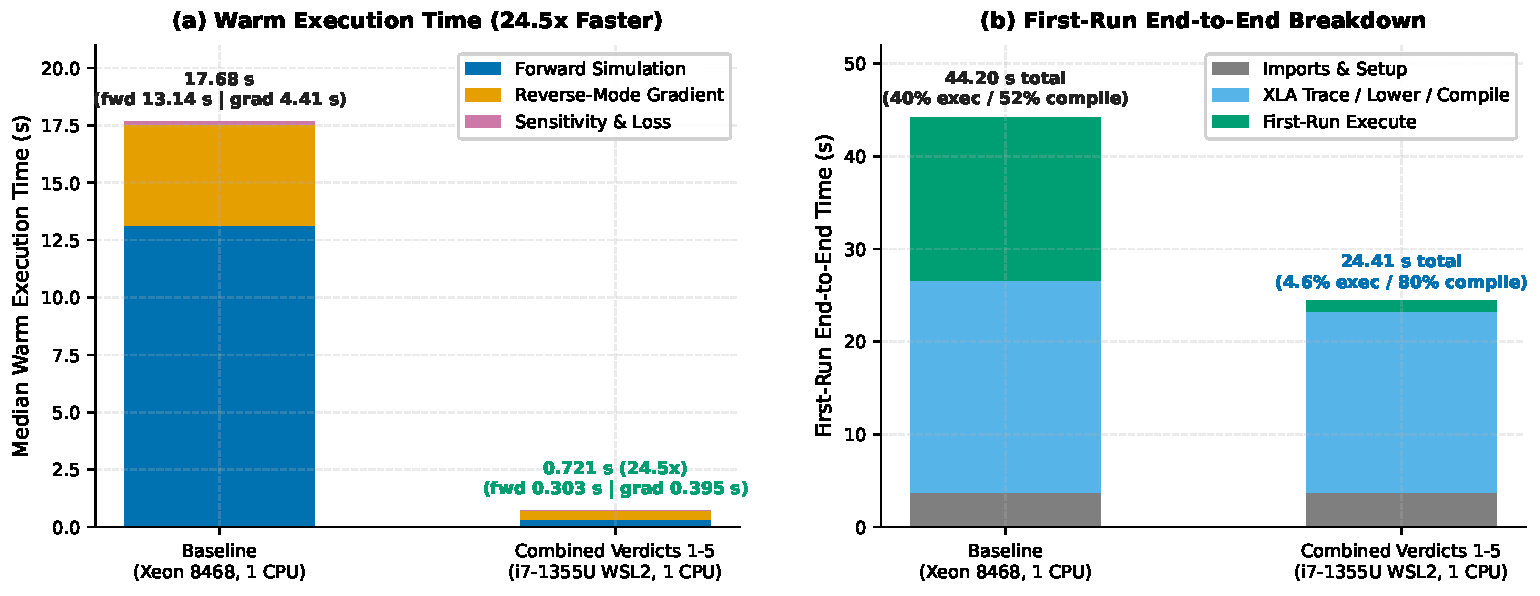
\includegraphics[width=\linewidth]{fig2_benchmark_comparison.pdf}
    \caption{Benchmark comparison on \texttt{uifo\_800\_3000} (1 logical CPU). (a)~Median warm execution drops from 17.68\,s to 0.721\,s ($24.5\times$ speedup). (b)~First-run end-to-end drops from 44.20\,s to 24.41\,s, leaving XLA compilation (19.60\,s, 80\%) as the dominant remaining bottleneck. Best viewed in color.}
    \label{fig:benchmarks}
\end{figure}

Figure~\ref{fig:benchmarks} and Table~\ref{tab:benchmarks} compare the baseline (\texttt{benchmarks/cpu-baseline.json}, Intel Xeon Platinum 8468, 1 CPU) against our combined implementation (\texttt{scratch/new3.json}, Intel Core i7-1355U WSL2, 1 CPU). \emph{Hardware caveat:} These two runs were measured on different CPUs, so single-thread IPC differences contribute alongside the algorithmic speedups; re-running both on the same judging Xeon machine is recommended for an apples-to-apples ratio.

\begin{table}[h]
\centering
\small
\begin{tabular}{@{}lrrr@{}}
\toprule
\textbf{Phase} & \textbf{Baseline (Xeon 8468)} & \textbf{Combined (i7-1355U)} & \textbf{Change} \\
\midrule
Imports \& Setup & 3.66\,s & 3.68\,s & $1.0\times$ \\
XLA Trace / Lower / Compile & 22.92\,s & 19.60\,s & $1.17\times$ \\
\midrule
Warm Forward (median) & 13.144\,s & 0.303\,s & \textbf{43.4$\times$ faster} \\
Warm Sensitivity (median) & 0.103\,s & 0.00053\,s & \textbf{194$\times$ faster} \\
Warm Gradient (median) & 4.411\,s & 0.395\,s & \textbf{11.2$\times$ faster} \\
\textbf{Warm Total (median)} & \textbf{17.679\,s} & \textbf{0.721\,s} & \textbf{24.5$\times$ faster} \\
\midrule
\textbf{First-Run End-to-End} & \textbf{44.204\,s} & \textbf{24.407\,s} & \textbf{1.81$\times$ faster} \\
\bottomrule
\end{tabular}
\caption{Phase-by-phase timing comparison on \texttt{uifo\_800\_3000} (1 logical CPU).}
\label{tab:benchmarks}
\end{table}

% ==============================================================================
\section{Causal Chain \& Glossary}
% ==============================================================================

\textbf{End-to-End Causal Chain:}
\begin{center}
\small
\fbox{\parbox{0.96\linewidth}{\centering
\textbf{1. Slim Dispatch (V5)} (4/4/15 branches) $\longrightarrow$
\textbf{2. Sparse COO Entries (V3)} (2,700 vs.\ 564k) $\longrightarrow$
\textbf{3. Cached SuperLU (V2)} (101 vs.\ 606 factorizations) $\longrightarrow$
\textbf{4. MISO Quadratic + Hoisted $N$ (V1+V4)} ($w^H N w$ at 760 nnz) $\longrightarrow$
\textbf{5. Sparse VJP (V3)} ($-\lambda_{r} x_{c}$, $209\times$ less work) $\longrightarrow$
\textbf{6. 0.721\,s Warm Runtime ($24.5\times$ faster)}
}}
\end{center}

\begin{table}[h]
\centering
\small
\begin{tabular}{@{}p{0.28\linewidth}p{0.66\linewidth}@{}}
\toprule
\textbf{Term} & \textbf{Plain Meaning} \\
\midrule
Carrier / Signal / Noise & Steady laser light ($286\times 286$), audio-band ripples ($751\times 751$), and quantum fluctuations ($751\times 751$). \\
Sparsity (0.48\% nnz) & Only $\sim$2,700 of 564,001 matrix entries are nonzero; the rest are blank zeros. \\
\texttt{splu} (SuperLU) & SciPy's C sparse LU solver that factors a matrix once and solves $A$, $A^T$, and $A^H$. \\
MISO Adjoint Identity & Rewriting $c^H A^{-1} N A^{-\dagger} c$ as $w^H N w$ ($w = A^{-\dagger} c$) to delete a redundant solve. \\
Sparse VJP ($-\lambda_r x_c$) & Computing reverse-mode matrix gradients only at nonzero coordinates, not densely. \\
\texttt{lax.switch} Slimming & Restricting each system to its 4 or 15 used component functions instead of all 19. \\
\bottomrule
\end{tabular}
\caption{Plain-language glossary of key concepts.}
\label{tab:glossary}
\end{table}

\end{document}
